\documentclass[12pt,]{article}
\usepackage{lmodern}
\usepackage{amssymb,amsmath}
\usepackage{ifxetex,ifluatex}
\usepackage{fixltx2e} % provides \textsubscript
\ifnum 0\ifxetex 1\fi\ifluatex 1\fi=0 % if pdftex
  \usepackage[T1]{fontenc}
  \usepackage[utf8]{inputenc}
\else % if luatex or xelatex
  \ifxetex
    \usepackage{mathspec}
  \else
    \usepackage{fontspec}
  \fi
  \defaultfontfeatures{Ligatures=TeX,Scale=MatchLowercase}
\fi
% use upquote if available, for straight quotes in verbatim environments
\IfFileExists{upquote.sty}{\usepackage{upquote}}{}
% use microtype if available
\IfFileExists{microtype.sty}{%
\usepackage{microtype}
\UseMicrotypeSet[protrusion]{basicmath} % disable protrusion for tt fonts
}{}
\usepackage[margin=1.0in]{geometry}
\usepackage{hyperref}
\hypersetup{unicode=true,
            pdftitle={Supplementary Information},
            pdfborder={0 0 0},
            breaklinks=true}
\urlstyle{same}  % don't use monospace font for urls
\usepackage{graphicx,grffile}
\makeatletter
\def\maxwidth{\ifdim\Gin@nat@width>\linewidth\linewidth\else\Gin@nat@width\fi}
\def\maxheight{\ifdim\Gin@nat@height>\textheight\textheight\else\Gin@nat@height\fi}
\makeatother
% Scale images if necessary, so that they will not overflow the page
% margins by default, and it is still possible to overwrite the defaults
% using explicit options in \includegraphics[width, height, ...]{}
\setkeys{Gin}{width=\maxwidth,height=\maxheight,keepaspectratio}
\IfFileExists{parskip.sty}{%
\usepackage{parskip}
}{% else
\setlength{\parindent}{0pt}
\setlength{\parskip}{6pt plus 2pt minus 1pt}
}
\setlength{\emergencystretch}{3em}  % prevent overfull lines
\providecommand{\tightlist}{%
  \setlength{\itemsep}{0pt}\setlength{\parskip}{0pt}}
\setcounter{secnumdepth}{0}
% Redefines (sub)paragraphs to behave more like sections
\ifx\paragraph\undefined\else
\let\oldparagraph\paragraph
\renewcommand{\paragraph}[1]{\oldparagraph{#1}\mbox{}}
\fi
\ifx\subparagraph\undefined\else
\let\oldsubparagraph\subparagraph
\renewcommand{\subparagraph}[1]{\oldsubparagraph{#1}\mbox{}}
\fi

%%% Use protect on footnotes to avoid problems with footnotes in titles
\let\rmarkdownfootnote\footnote%
\def\footnote{\protect\rmarkdownfootnote}

%%% Change title format to be more compact
\usepackage{titling}

% Create subtitle command for use in maketitle
\providecommand{\subtitle}[1]{
  \posttitle{
    \begin{center}\large#1\end{center}
    }
}

\setlength{\droptitle}{-2em}

  \title{\textbf{Supplementary Information}}
    \pretitle{\vspace{\droptitle}\centering\huge}
  \posttitle{\par}
  \subtitle{\textbf{Selective DNA and Protein Isolation from Marine Macrophyte
Surfaces}}
  \author{}
    \preauthor{}\postauthor{}
    \date{}
    \predate{}\postdate{}
  
\usepackage{times} % Times New Roman font
\usepackage[T1]{fontenc}

\usepackage[none]{hyphenat}

\usepackage{setspace}
\doublespacing
\setlength{\parskip}{1em}

\usepackage{lineno}

\usepackage{pdfpages}

\usepackage{indentfirst}

\usepackage[labelsep=period, labelfont=bf]{caption}
\renewcommand{\thefigure}{S\arabic{figure}}
\renewcommand{\figurename}{Fig.}
\renewcommand{\thetable}{S\arabic{table}}
\captionsetup{justification=raggedright,singlelinecheck=false}

\usepackage{pdflscape}
\newcommand{\blandscape}{\begin{landscape}}
\newcommand{\elandscape}{\end{landscape}}

\usepackage{siunitx}
\DeclareSIUnit\molar{\mole\per\cubic\deci\metre}
\DeclareSIUnit\Molar{\textsc{m}}
\DeclareSIUnit\cells{\text{cells}}

\usepackage{caption}
\captionsetup{justification=justified}

\usepackage{float}

\renewcommand{\figureautorefname}{Fig.}
\usepackage{booktabs}
\usepackage{longtable}
\usepackage{array}
\usepackage{multirow}
\usepackage{wrapfig}
\usepackage{float}
\usepackage{colortbl}
\usepackage{pdflscape}
\usepackage{tabu}
\usepackage{threeparttable}
\usepackage{threeparttablex}
\usepackage[normalem]{ulem}
\usepackage{makecell}
\usepackage{xcolor}

\begin{document}
\maketitle

\vspace{60mm}

Marino Korlević\textsuperscript{1\(*\)}, Marsej
Markovski\textsuperscript{1}, Zihao Zhao\textsuperscript{2}, Gerhard J.
Herndl\textsuperscript{2,3}, Mirjana Najdek\textsuperscript{1}

\vspace{40mm}

\textsuperscript{\(*\)}To whom correspondence should be addressed:
\href{mailto:marino.korlevic@irb.hr}{\nolinkurl{marino.korlevic@irb.hr}}

1. Center for Marine Research, Ruđer Bošković Institute, Croatia

2. Department of Functional and Evolutionary Ecology, University of
Vienna, Austria

3. Department of Marine Microbiology and Biogeochemistry, Royal
Netherlands Institute for Sea Research, Utrecht University, The
Netherlands

\sisetup{mode=text}
\setlength\parindent{24pt}

\hypertarget{supplementary-figures}{%
\subsection{Supplementary Figures}\label{supplementary-figures}}

\begin{figure}[H]

{\centering 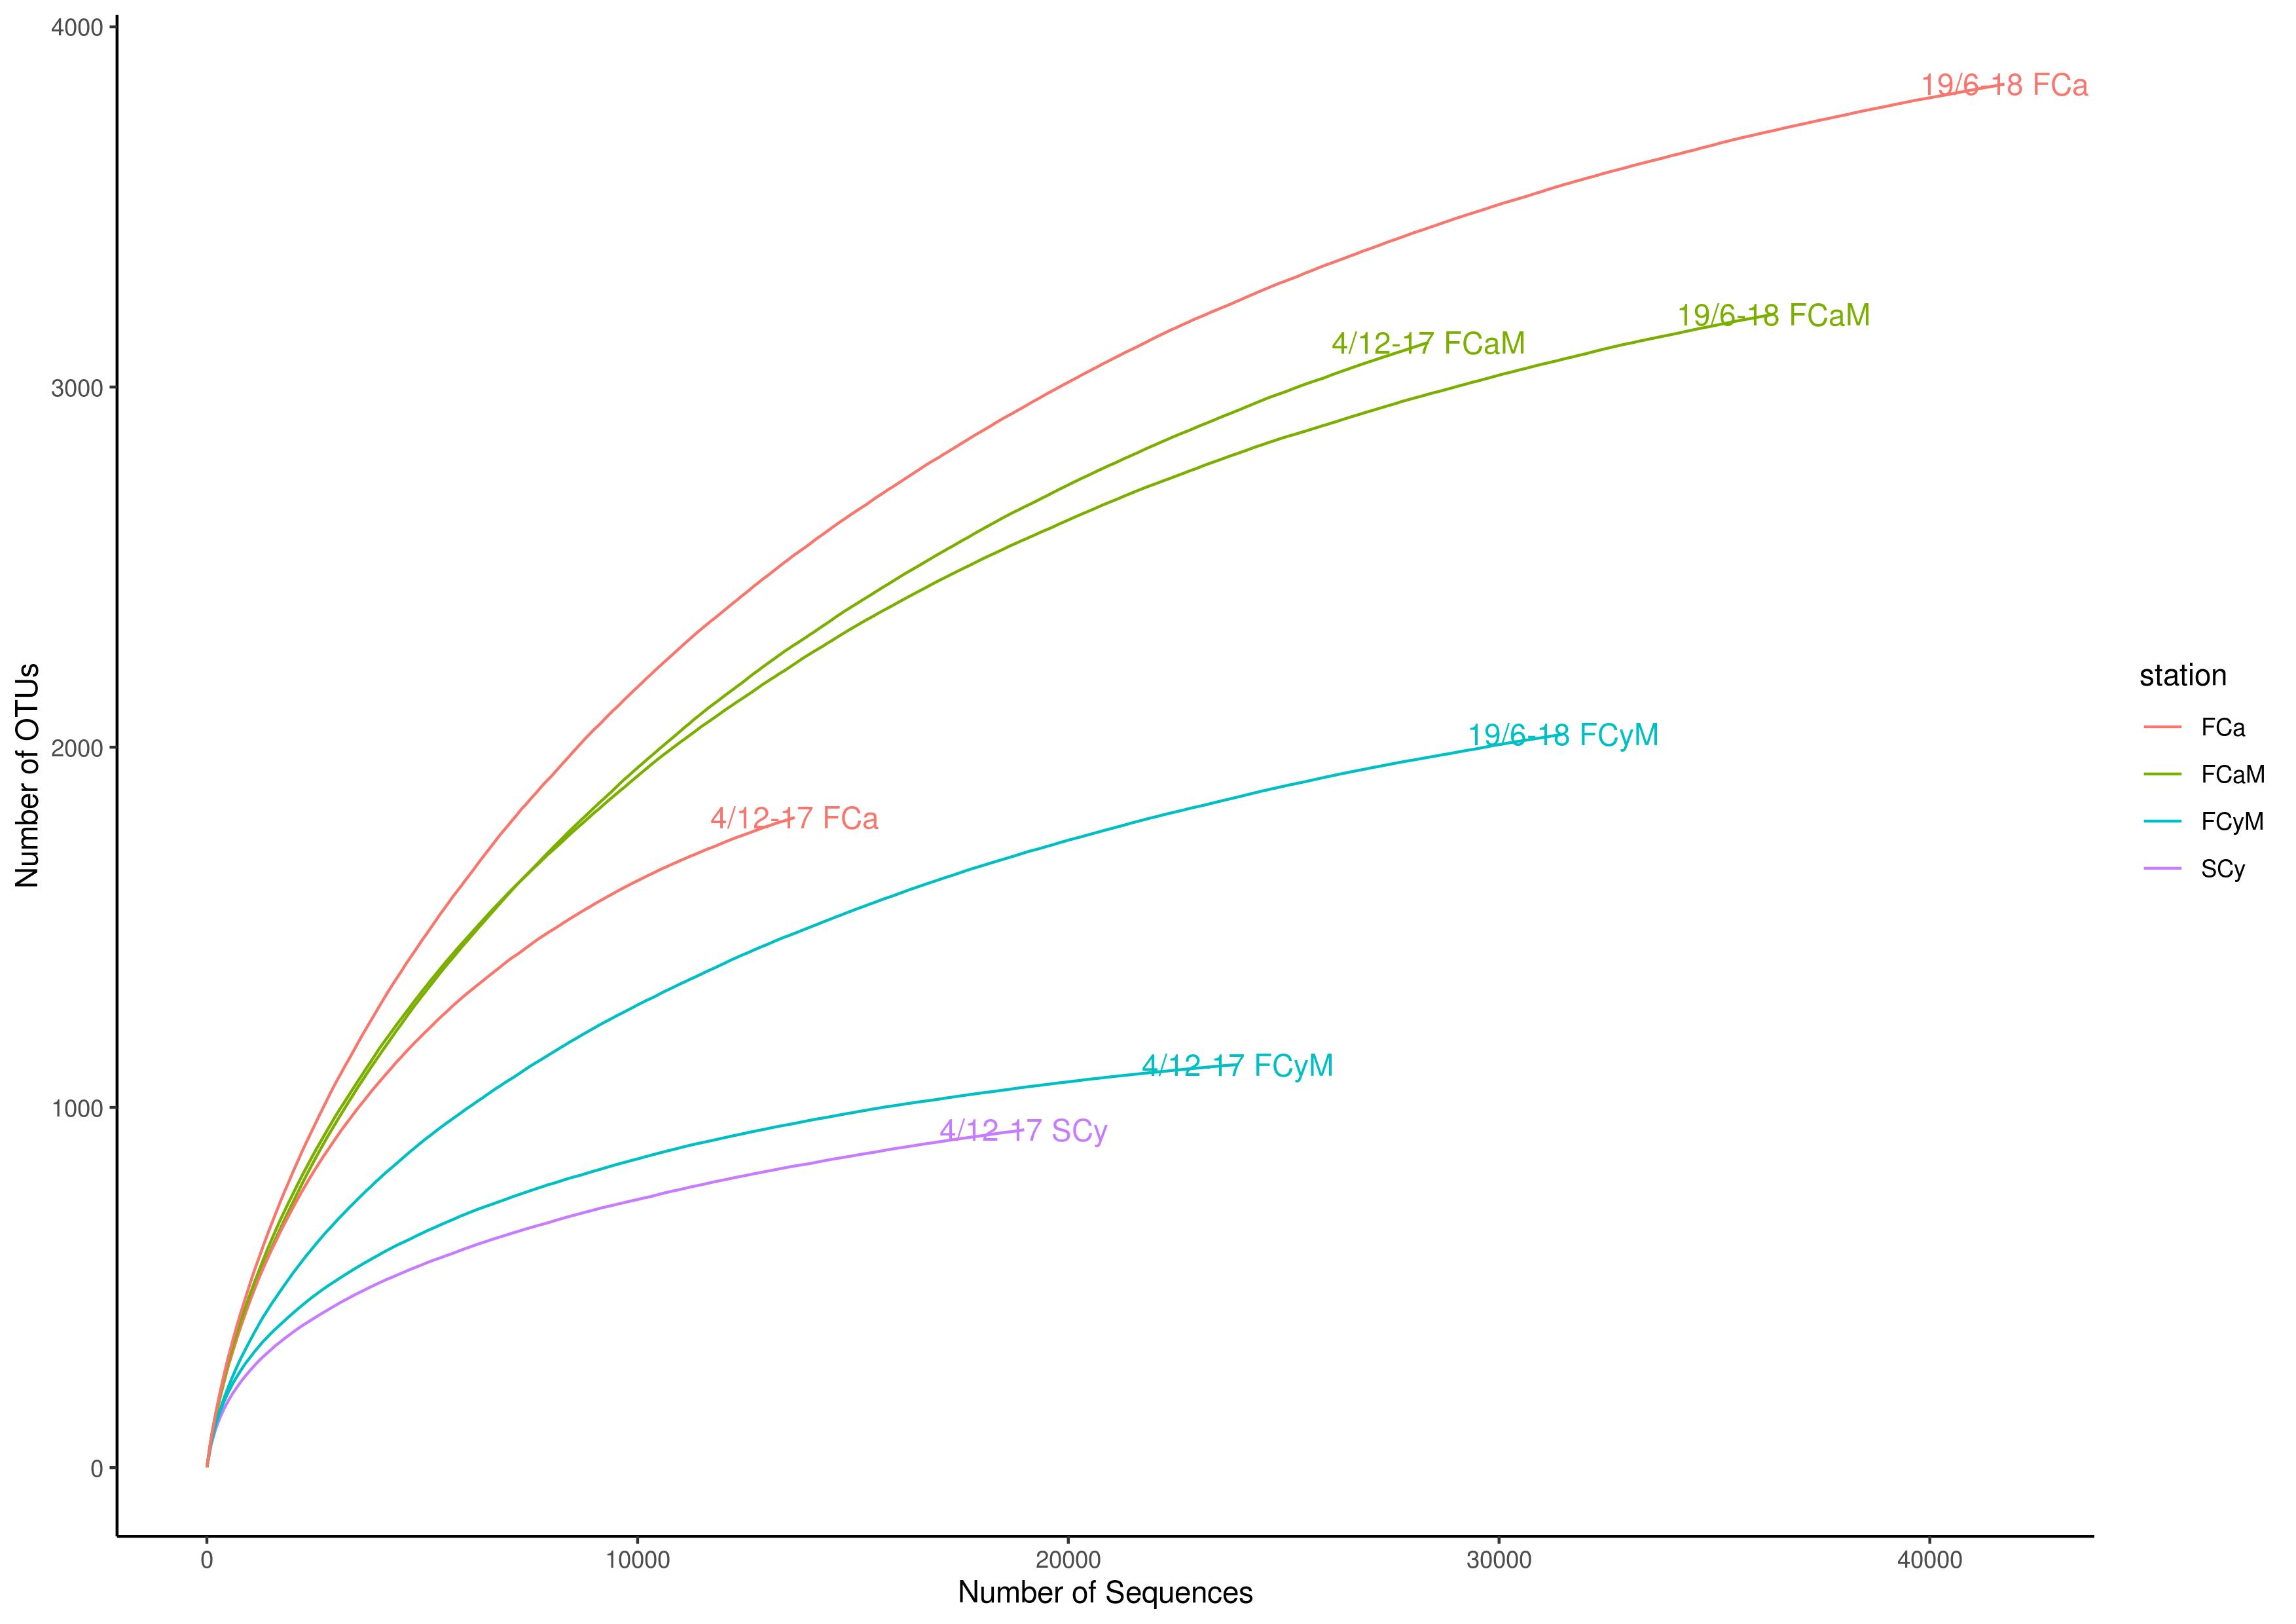
\includegraphics[width=0.8\linewidth]{../results/figures/rarefaction} 

}

\caption{Rarefaction curves of bacterial and archaeal communities from the surfaces of macrophytes sampled in the Bay of Saline (\textit{C. nodosa} [Monospecific Settlement]) and the Bay of Funatana (\textit{C. nodosa} [Mixed Settlement] and \textit{C. cylindracea} [Mixed and Monospecific Settlement]) in two contrasting seasons.\label{rarefaction}}\label{fig:unnamed-chunk-1}
\end{figure}

\newpage

\hypertarget{supplementary-table}{%
\subsection{Supplementary Table}\label{supplementary-table}}

\begingroup\fontsize{9}{11}\selectfont

\begin{longtable}[t]{>{\centering\arraybackslash}p{6em}ccccc}
\caption{\label{tab:nseq_notus}Sample ID, Station, Community Type, Sampling Date, No. of Sequences and No. of OTUs of each sample. No. of Sequences and OTUs was calculated after the exclusion of eukaryotic, chloroplast, mitochondrial and no relative sequences.\label{nseq_notus}}\\
\toprule
\textbf{Sample ID} & \textbf{Station} & \textbf{Community Type} & \textbf{Date} & \textbf{No. of Sequences} & \textbf{No. of OTUs}\\
\midrule
\endfirsthead
\caption[]{Sample ID, Station, Community Type, Sampling Date, No. of Sequences and No. of OTUs of each sample. No. of Sequences and OTUs was calculated after the exclusion of eukaryotic, chloroplast, mitochondrial and no relative sequences.\label{nseq_notus} \textit{(continued)}}\\
\toprule
\textbf{Sample ID} & \textbf{Station} & \textbf{Community Type} & \textbf{Date} & \textbf{No. of Sequences} & \textbf{No. of OTUs}\\
\midrule
\endhead
\
\endfoot
\bottomrule
\endlastfoot
40 & Saline & \textit{Cymodocea nodosa} (Monospecific) & 4 December 2017 & 19,178 & 938\\
41 & Funtana & \textit{Cymodocea nodosa} (Mixed) & 4 December 2017 & 24,248 & 1,119\\
42 & Funtana & \textit{Caulerpa cylindracea} (Mixed) & 4 December 2017 & 28,373 & 3,139\\
43 & Funtana & \textit{Caulerpa cylindracea} (Monospecific) & 4 December 2017 & 13,656 & 1,816\\
61 & Funtana & \textit{Cymodocea nodosa} (Mixed) & 19 June 2018 & 31,728 & 2,045\\
62 & Funtana & \textit{Caulerpa cylindracea} (Mixed) & 19 June 2018 & 36,484 & 3,225\\
63 & Funtana & \textit{Caulerpa cylindracea} (Monospecific) & 19 June 2018 & 41,840 & 3,861\\*
\end{longtable}
\endgroup{}


\end{document}
